%%%%%%%%%%%%%%%%%%%%%%%%%%%%%%%%%%%%%%%%%
% Beamer Presentation
% LaTeX Template
% Version 1.0 (10/11/12)
%
% This template has been downloaded from:
% http://www.LaTeXTemplates.com
%
% License:
% CC BY-NC-SA 3.0 (http://creativecommons.org/licenses/by-nc-sa/3.0/)
%
%%%%%%%%%%%%%%%%%%%%%%%%%%%%%%%%%%%%%%%%%

%----------------------------------------------------------------------------------------
%	PACKAGES AND THEMES
%----------------------------------------------------------------------------------------

\documentclass{beamer}

\mode<presentation> {

% The Beamer class comes with a number of default slide themes
% which change the colors and layouts of slides. Below this is a list
% of all the themes, uncomment each in turn to see what they look like.

%\usetheme{default}
%\usetheme{AnnArbor}
%\usetheme{Antibes}
%\usetheme{Bergen}
%\usetheme{Berkeley}
%\usetheme{Berlin}
%\usetheme{Boadilla}
%\usetheme{CambridgeUS}
%\usetheme{Copenhagen}
%\usetheme{Darmstadt}
%\usetheme{Dresden}
%\usetheme{Frankfurt}
%\usetheme{Goettingen}
%\usetheme{Hannover}
%\usetheme{Ilmenau}
%\usetheme{JuanLesPins}
%\usetheme{Luebeck}
%\usetheme{Madrid}
%\usetheme{Malmoe}
%\usetheme{Marburg}
%\usetheme{Montpellier}
\usetheme{PaloAlto}
%\usetheme{Pittsburgh}
%\usetheme{Rochester}
%\usetheme{Singapore}
%\usetheme{Szeged}
%\usetheme{Warsaw}

% As well as themes, the Beamer class has a number of color themes
% for any slide theme. Uncomment each of these in turn to see how it
% changes the colors of your current slide theme.

%\usecolortheme{albatross}
%\usecolortheme{beaver}
%\usecolortheme{beetle}
%\usecolortheme{crane}
%\usecolortheme{dolphin}
%\usecolortheme{dove}
%\usecolortheme{fly}
%\usecolortheme{lily}
\usecolortheme{orchid}
%\usecolortheme{rose}
%\usecolortheme{seagull}
%\usecolortheme{seahorse}
%\usecolortheme{whale}
%\usecolortheme{wolverine}

%\setbeamertemplate{footline} % To remove the footer line in all slides uncomment this line
%\setbeamertemplate{footline}[page number] % To replace the footer line in all slides with a simple slide count uncomment this line

%\setbeamertemplate{navigation symbols}{} % To remove the navigation symbols from the bottom of all slides uncomment this line
}

\usepackage{graphicx} % Allows including images
\usepackage{times,epsfig}
\usepackage{epstopdf}
\usepackage{booktabs} % Allows the use of \toprule, \midrule and \bottomrule in tables

%----------------------------------------------------------------------------------------
%	TITLE PAGE
%----------------------------------------------------------------------------------------

\title[Experimental Results]{Analysis of Networks} % The short title appears at the bottom of every slide, the full title is only on the title page

\author{Tao Wang} % Your name
\institute[Soton] % Your institution as it will appear on the bottom of every slide, may be shorthand to save space
{
University of Southampton \\ % Your institution for the title page
\medskip
\textit{t.wang@soton.ac.uk} % Your email address
}
\date{\today} % Date, can be changed to a custom date

\begin{document}

\begin{frame}
\titlepage % Print the title page as the first slide
\end{frame}

%\begin{frame}
%\frametitle{Overview} % Table of contents slide, comment this block out to remove it
%\tableofcontents % Throughout your presentation, if you choose to use \section{} and \subsection{} commands, these will automatically be printed on this slide as an overview of your presentation
%\end{frame}

%----------------------------------------------------------------------------------------
%	PRESENTATION SLIDES
%----------------------------------------------------------------------------------------

%------------------------------------------------
%\section{First Section} % Sections can be created in order to organize your presentation into discrete blocks, all sections and subsections are automatically printed in the table of contents as an overview of the talk
%%------------------------------------------------
%
%\subsection{Subsection Example} % A subsection can be created just before a set of slides with a common theme to further break down your presentation into chunks



\begin{frame}
\frametitle{Distribution of Link Weights}
\begin{figure}
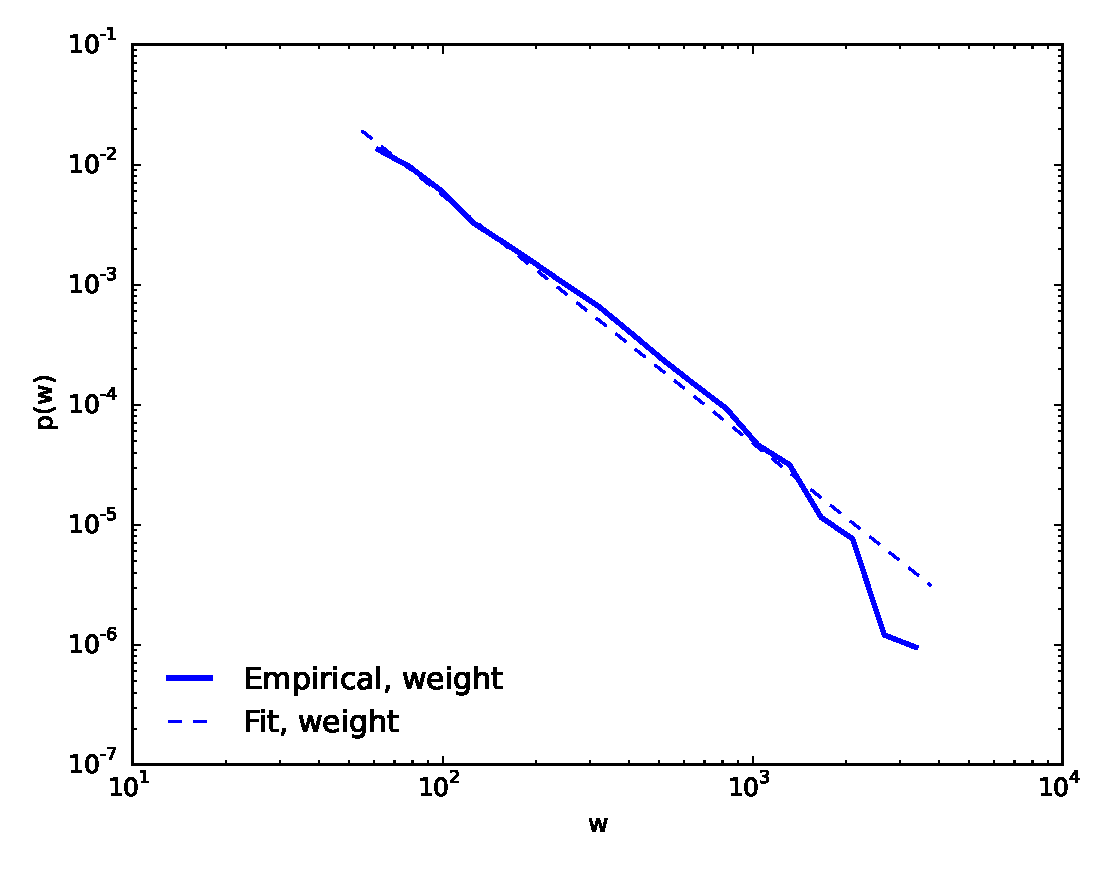
\includegraphics[width=0.65\linewidth]{wpdf.eps}
\end{figure}
\small{The figure is the probability density function (PDF) of the $W$ matrix, including in-strength and out-strength, where $\alpha=2.05$ and standard error (i.e., RMSE) $\sigma= 0.029$ (The power-law distributions are formulated with: $p(x)\propto x^{-\alpha}$).}
\end{frame}





\begin{frame}
\frametitle{Distribution of Strength}
\begin{figure}
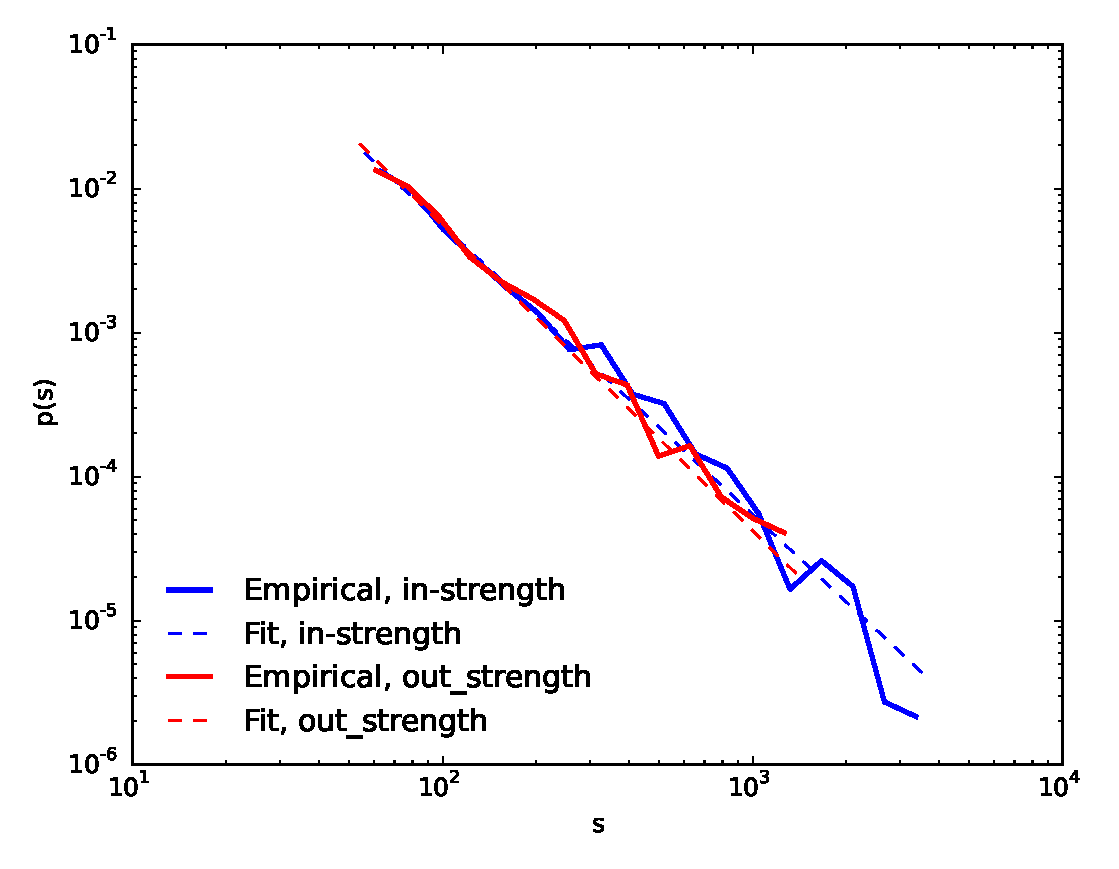
\includegraphics[width=0.65\linewidth]{strengthpdf.eps}
\end{figure}
\small{The figure is obtained by in/out strength plus one. The PDF of in-strength are fitted by a power-law with $\alpha=2.01$ and $\sigma=0.041$. The PDF of out-strength are fitted by a power-law with $\alpha=2.12$ and $\sigma=0.041$.
}
\end{frame}


\begin{frame}
\frametitle{Distribution of Degrees}
\begin{figure}
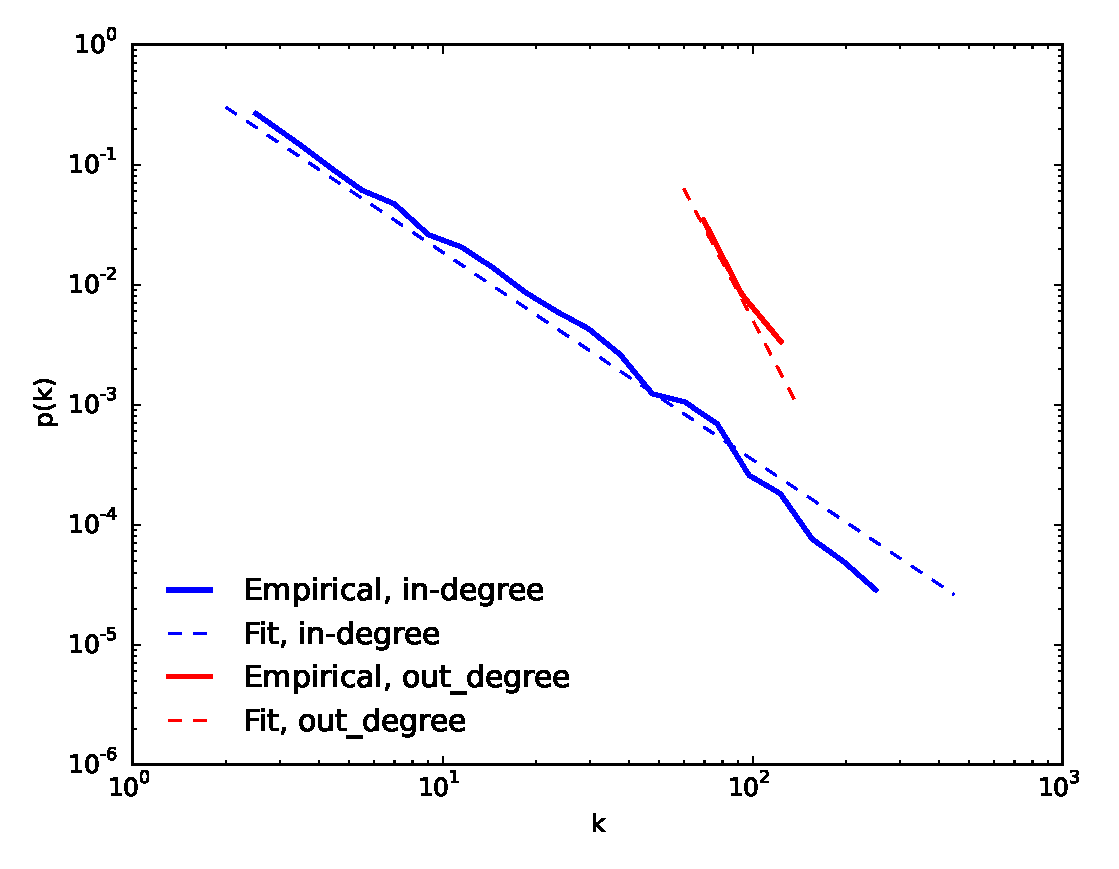
\includegraphics[width=0.65\linewidth]{degreepdf.eps}
\end{figure}
\small{The figure is obtained by in/out degrees plus one. The probability density function (PDF) of in-degrees are fitted by a power-law with $\alpha=1.73$ and $\sigma=0.012$. The PDF of out-degrees are fitted by a power-law with $\alpha=4.92$ and $\sigma=0.423$.}
\end{frame}

\begin{frame}
\frametitle{Dependence of Strength and Degrees}
\begin{figure}
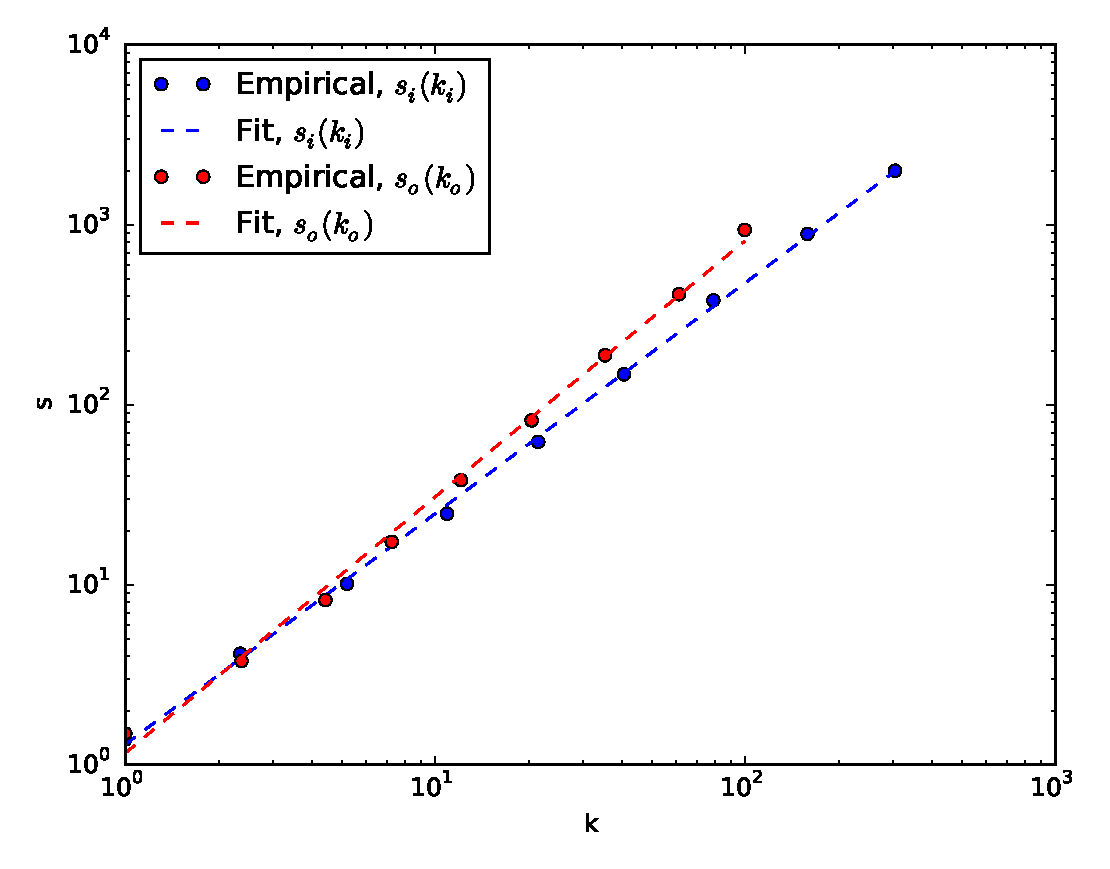
\includegraphics[width=0.65\linewidth]{sd.eps}
\end{figure}
\small{The figure is obtained by in/out degrees and in-out degrees plus one. The dependence of in-strength and in-degrees are fitted by a power-law with $\alpha=1.282$ and $\sigma=0.027$. The PDF of out-degrees are fitted by a power-law with $\alpha=1.424$ and $\sigma=0.052$.}
\end{frame}

\begin{frame}
\frametitle{Dependence of In-degrees and Out-degrees}
\begin{figure}
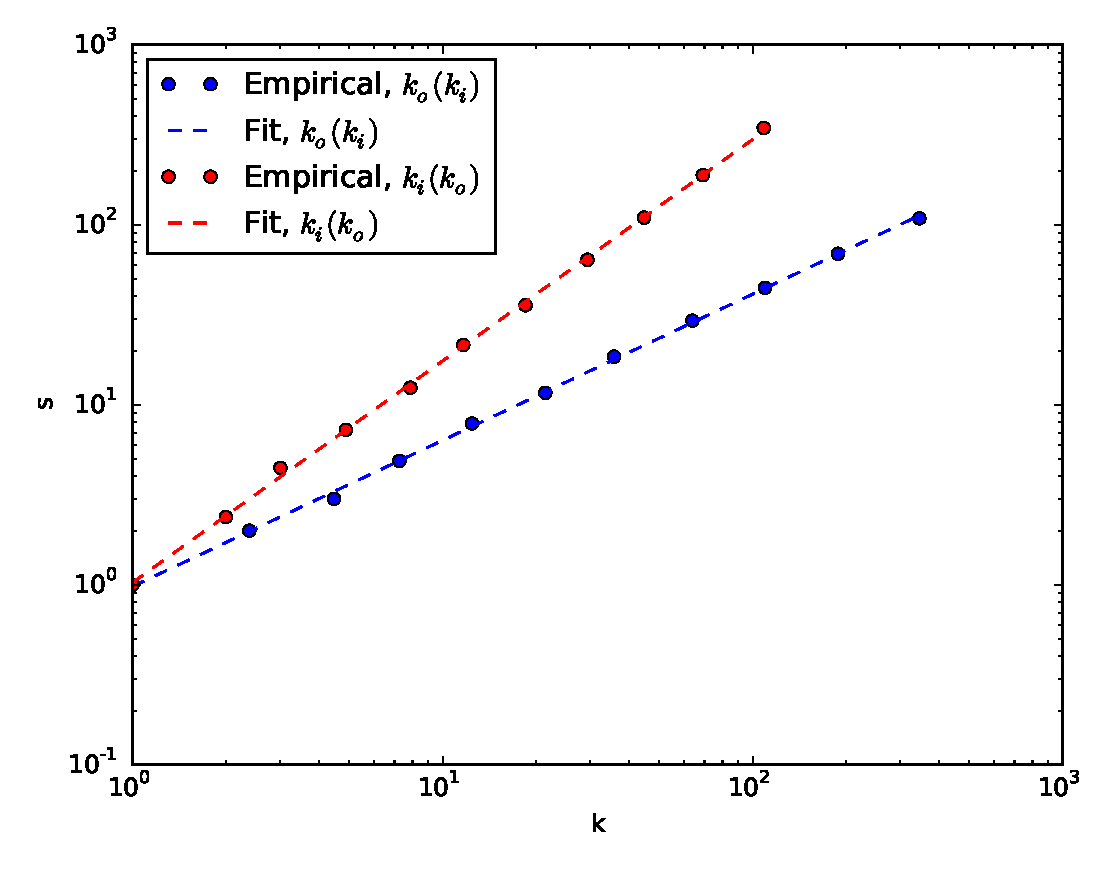
\includegraphics[width=0.65\linewidth]{dd.eps}
\end{figure}
\small{The figure is obtained by in/out degrees (without plus one). The $k_o(k_i)$ fitted by a power-law with $\alpha=0.8121$ and $\sigma=0.016$. The $k_i(k_o)$ is fitted by a power-law with $\alpha=1.231$ and $\sigma=0.019$.}
\end{frame}


\begin{frame}
\frametitle{Dependence of In-strength and Out-strength}
\begin{figure}
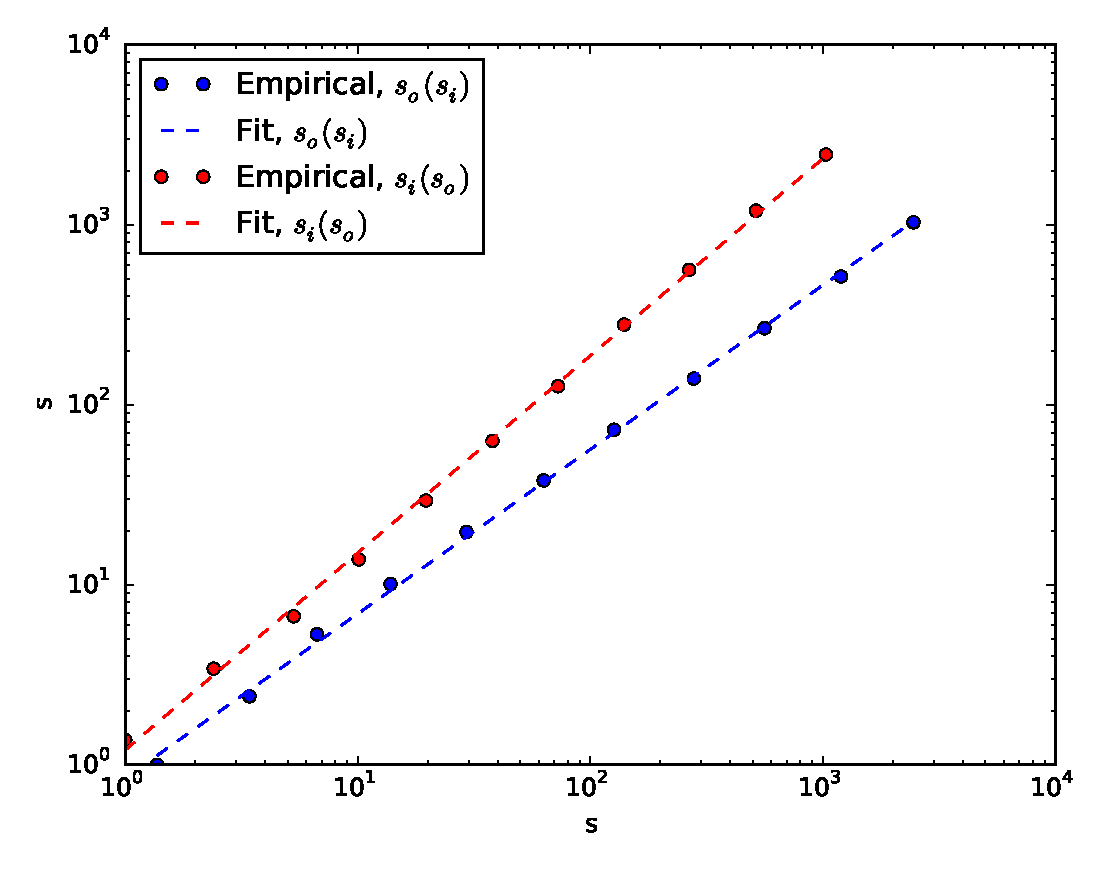
\includegraphics[width=0.65\linewidth]{ss.eps}
\end{figure}
\small{The figure is obtained by in/out strength (without plus one). The $s_o(s_i)$ fitted by a power-law with $\alpha=0.9123$ and $\sigma=0.028$. The $s_i(s_o)$ is fitted by a power-law with $\alpha=1.095$ and $\sigma=0.031$.}
\end{frame}

%------------------------------------------------

\begin{frame}
\Huge{\centerline{The End}}
\end{frame}

%----------------------------------------------------------------------------------------

\end{document} 